\begin{frame}{taint tracking assembly?}
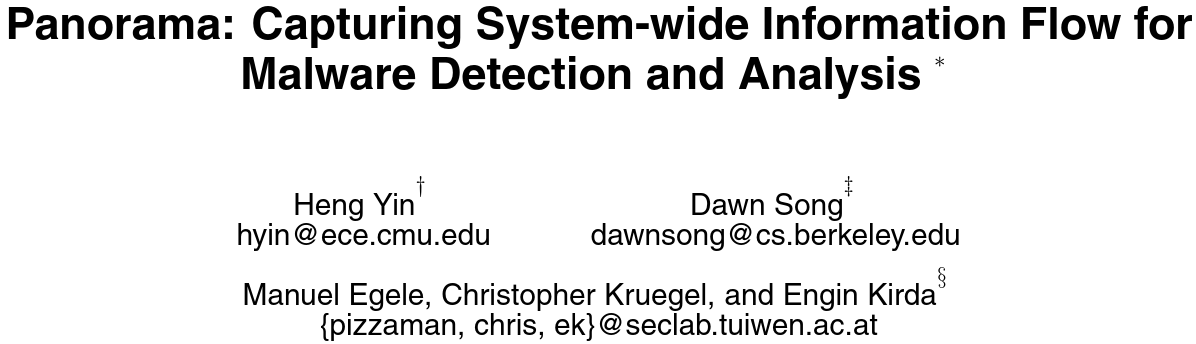
\includegraphics[width=\textwidth]{../taint/panaroma}
\end{frame}

\begin{frame}{high-level overview}
\begin{itemize}
\item lookup table for each register and byte of memory:
    \begin{itemize}
    \item where did this value come from?
    \end{itemize}
\item \texttt{add \%r9, (\%r8)}: \\
    \texttt{memory-taint-table[register-values[R8]] =} \\
    \hspace{4cm} \texttt{register-taint-table[R9]}
\item also similar for virtual disk, network, \ldots
\item custom VM: all applications and the OS run with taint tracking
\end{itemize}
\end{frame}

\begin{frame}[fragile,label=panaromaSpecial]{Panaroma special cases}
\begin{itemize}
\item \texttt{xor \%eax, \%eax}: special case: remove taint from \%eax
\item Windows keyboard input did something like:
\begin{lstlisting}
keycode = GetFromKeyboard();
switch (keycode) {
case KEYCODE_A: return 'a';
case KEYCODE_B: return 'b';
...
}
\end{lstlisting}
\end{itemize}
\end{frame}

\begin{frame}{taint tracking for malware analysis}
\begin{itemize}
\item uses proposed by Panaroma authors:
\vspace{.5cm}
\item keypresses $\rightarrow$ network packets
\item network packets $\rightarrow$ malware outputs
\item browser history $\rightarrow$ network packets
\end{itemize}
\end{frame}
